% Options for packages loaded elsewhere
\PassOptionsToPackage{unicode}{hyperref}
\PassOptionsToPackage{hyphens}{url}
\PassOptionsToPackage{dvipsnames,svgnames,x11names}{xcolor}
%
\documentclass[
  letterpaper,
  DIV=11,
  numbers=noendperiod]{scrartcl}

\usepackage{amsmath,amssymb}
\usepackage{lmodern}
\usepackage{iftex}
\ifPDFTeX
  \usepackage[T1]{fontenc}
  \usepackage[utf8]{inputenc}
  \usepackage{textcomp} % provide euro and other symbols
\else % if luatex or xetex
  \usepackage{unicode-math}
  \defaultfontfeatures{Scale=MatchLowercase}
  \defaultfontfeatures[\rmfamily]{Ligatures=TeX,Scale=1}
\fi
% Use upquote if available, for straight quotes in verbatim environments
\IfFileExists{upquote.sty}{\usepackage{upquote}}{}
\IfFileExists{microtype.sty}{% use microtype if available
  \usepackage[]{microtype}
  \UseMicrotypeSet[protrusion]{basicmath} % disable protrusion for tt fonts
}{}
\makeatletter
\@ifundefined{KOMAClassName}{% if non-KOMA class
  \IfFileExists{parskip.sty}{%
    \usepackage{parskip}
  }{% else
    \setlength{\parindent}{0pt}
    \setlength{\parskip}{6pt plus 2pt minus 1pt}}
}{% if KOMA class
  \KOMAoptions{parskip=half}}
\makeatother
\usepackage{xcolor}
\setlength{\emergencystretch}{3em} % prevent overfull lines
\setcounter{secnumdepth}{-\maxdimen} % remove section numbering
% Make \paragraph and \subparagraph free-standing
\ifx\paragraph\undefined\else
  \let\oldparagraph\paragraph
  \renewcommand{\paragraph}[1]{\oldparagraph{#1}\mbox{}}
\fi
\ifx\subparagraph\undefined\else
  \let\oldsubparagraph\subparagraph
  \renewcommand{\subparagraph}[1]{\oldsubparagraph{#1}\mbox{}}
\fi

\usepackage{color}
\usepackage{fancyvrb}
\newcommand{\VerbBar}{|}
\newcommand{\VERB}{\Verb[commandchars=\\\{\}]}
\DefineVerbatimEnvironment{Highlighting}{Verbatim}{commandchars=\\\{\}}
% Add ',fontsize=\small' for more characters per line
\usepackage{framed}
\definecolor{shadecolor}{RGB}{241,243,245}
\newenvironment{Shaded}{\begin{snugshade}}{\end{snugshade}}
\newcommand{\AlertTok}[1]{\textcolor[rgb]{0.68,0.00,0.00}{#1}}
\newcommand{\AnnotationTok}[1]{\textcolor[rgb]{0.37,0.37,0.37}{#1}}
\newcommand{\AttributeTok}[1]{\textcolor[rgb]{0.40,0.45,0.13}{#1}}
\newcommand{\BaseNTok}[1]{\textcolor[rgb]{0.68,0.00,0.00}{#1}}
\newcommand{\BuiltInTok}[1]{\textcolor[rgb]{0.00,0.23,0.31}{#1}}
\newcommand{\CharTok}[1]{\textcolor[rgb]{0.13,0.47,0.30}{#1}}
\newcommand{\CommentTok}[1]{\textcolor[rgb]{0.37,0.37,0.37}{#1}}
\newcommand{\CommentVarTok}[1]{\textcolor[rgb]{0.37,0.37,0.37}{\textit{#1}}}
\newcommand{\ConstantTok}[1]{\textcolor[rgb]{0.56,0.35,0.01}{#1}}
\newcommand{\ControlFlowTok}[1]{\textcolor[rgb]{0.00,0.23,0.31}{#1}}
\newcommand{\DataTypeTok}[1]{\textcolor[rgb]{0.68,0.00,0.00}{#1}}
\newcommand{\DecValTok}[1]{\textcolor[rgb]{0.68,0.00,0.00}{#1}}
\newcommand{\DocumentationTok}[1]{\textcolor[rgb]{0.37,0.37,0.37}{\textit{#1}}}
\newcommand{\ErrorTok}[1]{\textcolor[rgb]{0.68,0.00,0.00}{#1}}
\newcommand{\ExtensionTok}[1]{\textcolor[rgb]{0.00,0.23,0.31}{#1}}
\newcommand{\FloatTok}[1]{\textcolor[rgb]{0.68,0.00,0.00}{#1}}
\newcommand{\FunctionTok}[1]{\textcolor[rgb]{0.28,0.35,0.67}{#1}}
\newcommand{\ImportTok}[1]{\textcolor[rgb]{0.00,0.46,0.62}{#1}}
\newcommand{\InformationTok}[1]{\textcolor[rgb]{0.37,0.37,0.37}{#1}}
\newcommand{\KeywordTok}[1]{\textcolor[rgb]{0.00,0.23,0.31}{#1}}
\newcommand{\NormalTok}[1]{\textcolor[rgb]{0.00,0.23,0.31}{#1}}
\newcommand{\OperatorTok}[1]{\textcolor[rgb]{0.37,0.37,0.37}{#1}}
\newcommand{\OtherTok}[1]{\textcolor[rgb]{0.00,0.23,0.31}{#1}}
\newcommand{\PreprocessorTok}[1]{\textcolor[rgb]{0.68,0.00,0.00}{#1}}
\newcommand{\RegionMarkerTok}[1]{\textcolor[rgb]{0.00,0.23,0.31}{#1}}
\newcommand{\SpecialCharTok}[1]{\textcolor[rgb]{0.37,0.37,0.37}{#1}}
\newcommand{\SpecialStringTok}[1]{\textcolor[rgb]{0.13,0.47,0.30}{#1}}
\newcommand{\StringTok}[1]{\textcolor[rgb]{0.13,0.47,0.30}{#1}}
\newcommand{\VariableTok}[1]{\textcolor[rgb]{0.07,0.07,0.07}{#1}}
\newcommand{\VerbatimStringTok}[1]{\textcolor[rgb]{0.13,0.47,0.30}{#1}}
\newcommand{\WarningTok}[1]{\textcolor[rgb]{0.37,0.37,0.37}{\textit{#1}}}

\providecommand{\tightlist}{%
  \setlength{\itemsep}{0pt}\setlength{\parskip}{0pt}}\usepackage{longtable,booktabs,array}
\usepackage{calc} % for calculating minipage widths
% Correct order of tables after \paragraph or \subparagraph
\usepackage{etoolbox}
\makeatletter
\patchcmd\longtable{\par}{\if@noskipsec\mbox{}\fi\par}{}{}
\makeatother
% Allow footnotes in longtable head/foot
\IfFileExists{footnotehyper.sty}{\usepackage{footnotehyper}}{\usepackage{footnote}}
\makesavenoteenv{longtable}
\usepackage{graphicx}
\makeatletter
\def\maxwidth{\ifdim\Gin@nat@width>\linewidth\linewidth\else\Gin@nat@width\fi}
\def\maxheight{\ifdim\Gin@nat@height>\textheight\textheight\else\Gin@nat@height\fi}
\makeatother
% Scale images if necessary, so that they will not overflow the page
% margins by default, and it is still possible to overwrite the defaults
% using explicit options in \includegraphics[width, height, ...]{}
\setkeys{Gin}{width=\maxwidth,height=\maxheight,keepaspectratio}
% Set default figure placement to htbp
\makeatletter
\def\fps@figure{htbp}
\makeatother

\KOMAoption{captions}{tableheading}
\makeatletter
\makeatother
\makeatletter
\makeatother
\makeatletter
\@ifpackageloaded{caption}{}{\usepackage{caption}}
\AtBeginDocument{%
\ifdefined\contentsname
  \renewcommand*\contentsname{Table of contents}
\else
  \newcommand\contentsname{Table of contents}
\fi
\ifdefined\listfigurename
  \renewcommand*\listfigurename{List of Figures}
\else
  \newcommand\listfigurename{List of Figures}
\fi
\ifdefined\listtablename
  \renewcommand*\listtablename{List of Tables}
\else
  \newcommand\listtablename{List of Tables}
\fi
\ifdefined\figurename
  \renewcommand*\figurename{Figure}
\else
  \newcommand\figurename{Figure}
\fi
\ifdefined\tablename
  \renewcommand*\tablename{Table}
\else
  \newcommand\tablename{Table}
\fi
}
\@ifpackageloaded{float}{}{\usepackage{float}}
\floatstyle{ruled}
\@ifundefined{c@chapter}{\newfloat{codelisting}{h}{lop}}{\newfloat{codelisting}{h}{lop}[chapter]}
\floatname{codelisting}{Listing}
\newcommand*\listoflistings{\listof{codelisting}{List of Listings}}
\makeatother
\makeatletter
\@ifpackageloaded{caption}{}{\usepackage{caption}}
\@ifpackageloaded{subcaption}{}{\usepackage{subcaption}}
\makeatother
\makeatletter
\@ifpackageloaded{tcolorbox}{}{\usepackage[many]{tcolorbox}}
\makeatother
\makeatletter
\@ifundefined{shadecolor}{\definecolor{shadecolor}{rgb}{.97, .97, .97}}
\makeatother
\makeatletter
\makeatother
\ifLuaTeX
  \usepackage{selnolig}  % disable illegal ligatures
\fi
\IfFileExists{bookmark.sty}{\usepackage{bookmark}}{\usepackage{hyperref}}
\IfFileExists{xurl.sty}{\usepackage{xurl}}{} % add URL line breaks if available
\urlstyle{same} % disable monospaced font for URLs
\hypersetup{
  pdftitle={STAT570-HW2},
  pdfauthor={Oğuzhan Aydın},
  colorlinks=true,
  linkcolor={blue},
  filecolor={Maroon},
  citecolor={Blue},
  urlcolor={Blue},
  pdfcreator={LaTeX via pandoc}}

\title{STAT570-HW2}
\author{Oğuzhan Aydın}
\date{}

\begin{document}
\maketitle
\ifdefined\Shaded\renewenvironment{Shaded}{\begin{tcolorbox}[interior hidden, boxrule=0pt, borderline west={3pt}{0pt}{shadecolor}, sharp corners, breakable, enhanced, frame hidden]}{\end{tcolorbox}}\fi

\begin{Shaded}
\begin{Highlighting}[]
\FunctionTok{library}\NormalTok{(tidyverse) }
\end{Highlighting}
\end{Shaded}

\begin{verbatim}
-- Attaching core tidyverse packages ------------------------ tidyverse 2.0.0 --
v dplyr     1.1.2     v readr     2.1.4
v forcats   1.0.0     v stringr   1.5.0
v ggplot2   3.4.2     v tibble    3.2.1
v lubridate 1.9.2     v tidyr     1.3.0
v purrr     1.0.1     
-- Conflicts ------------------------------------------ tidyverse_conflicts() --
x dplyr::filter() masks stats::filter()
x dplyr::lag()    masks stats::lag()
i Use the conflicted package (<http://conflicted.r-lib.org/>) to force all conflicts to become errors
\end{verbatim}

\begin{Shaded}
\begin{Highlighting}[]
\FunctionTok{library}\NormalTok{(dplyr) }
\FunctionTok{library}\NormalTok{(nycflights13) }
\end{Highlighting}
\end{Shaded}

\begin{verbatim}
Warning: package 'nycflights13' was built under R version 4.3.1
\end{verbatim}

\begin{Shaded}
\begin{Highlighting}[]
\NormalTok{make\_datetime\_100 }\OtherTok{\textless{}{-}} \ControlFlowTok{function}\NormalTok{(year, month, day, time) \{}
  \FunctionTok{make\_datetime}\NormalTok{(year, month, day, time }\SpecialCharTok{\%/\%} \DecValTok{100}\NormalTok{, time }\SpecialCharTok{\%\%} \DecValTok{100}\NormalTok{)}
\NormalTok{  \} }
\NormalTok{flights\_dt }\OtherTok{\textless{}{-}}\NormalTok{ flights }\SpecialCharTok{|\textgreater{}}
  \FunctionTok{filter}\NormalTok{(}\SpecialCharTok{!}\FunctionTok{is.na}\NormalTok{(dep\_time), }\SpecialCharTok{!}\FunctionTok{is.na}\NormalTok{(arr\_time)) }\SpecialCharTok{|\textgreater{}}
  \FunctionTok{mutate}\NormalTok{(}
    \AttributeTok{dep\_time =} \FunctionTok{make\_datetime\_100}\NormalTok{(year, month, day, dep\_time),}
    \AttributeTok{arr\_time =} \FunctionTok{make\_datetime\_100}\NormalTok{(year, month, day, arr\_time),}
    \AttributeTok{sched\_dep\_time =} \FunctionTok{make\_datetime\_100}\NormalTok{(year, month, day, sched\_dep\_time),}
    \AttributeTok{sched\_arr\_time =} \FunctionTok{make\_datetime\_100}\NormalTok{(year, month, day, sched\_arr\_time)}
\NormalTok{    ) }\SpecialCharTok{|\textgreater{}}    
  \FunctionTok{select}\NormalTok{(origin, dest, }\FunctionTok{ends\_with}\NormalTok{(}\StringTok{"delay"}\NormalTok{), }\FunctionTok{ends\_with}\NormalTok{(}\StringTok{"time"}\NormalTok{))}
\NormalTok{flights\_dt2 }\OtherTok{\textless{}{-}}\NormalTok{ flights\_dt}
\end{Highlighting}
\end{Shaded}

\hypertarget{from-other-types}{%
\subsection{\texorpdfstring{17.2.4 \textbf{From other
types}}{17.2.4 From other types}}\label{from-other-types}}

By writing the following codes, we can get today's date and the exact
time for now.

\begin{Shaded}
\begin{Highlighting}[]
\FunctionTok{today}\NormalTok{() }
\end{Highlighting}
\end{Shaded}

\begin{verbatim}
[1] "2023-11-21"
\end{verbatim}

\begin{Shaded}
\begin{Highlighting}[]
\FunctionTok{now}\NormalTok{()}
\end{Highlighting}
\end{Shaded}

\begin{verbatim}
[1] "2023-11-21 21:52:15 +03"
\end{verbatim}

Additionally, by changing the time zone, we can reach the current time
or specific time in any part of the world.

\begin{Shaded}
\begin{Highlighting}[]
\FunctionTok{as\_datetime}\NormalTok{(}\FunctionTok{now}\NormalTok{(), }\AttributeTok{tz=}\StringTok{"UTC"}\NormalTok{) }
\end{Highlighting}
\end{Shaded}

\begin{verbatim}
[1] "2023-11-21 18:52:16 UTC"
\end{verbatim}

\begin{Shaded}
\begin{Highlighting}[]
\FunctionTok{as\_datetime}\NormalTok{(}\FunctionTok{now}\NormalTok{(), }\AttributeTok{tz=}\StringTok{"Europe/Istanbul"}\NormalTok{) }
\end{Highlighting}
\end{Shaded}

\begin{verbatim}
[1] "2023-11-21 21:52:16 +03"
\end{verbatim}

\begin{Shaded}
\begin{Highlighting}[]
\FunctionTok{as\_datetime}\NormalTok{(}\FunctionTok{now}\NormalTok{(), }\AttributeTok{tz=}\StringTok{"Europe/Paris"}\NormalTok{) }
\end{Highlighting}
\end{Shaded}

\begin{verbatim}
[1] "2023-11-21 19:52:16 CET"
\end{verbatim}

\begin{Shaded}
\begin{Highlighting}[]
\FunctionTok{as.POSIXct}\NormalTok{(}\FunctionTok{now}\NormalTok{(), }\AttributeTok{tz =} \StringTok{"CET"}\NormalTok{) }
\end{Highlighting}
\end{Shaded}

\begin{verbatim}
[1] "2023-11-21 19:52:16 CET"
\end{verbatim}

\begin{Shaded}
\begin{Highlighting}[]
\FunctionTok{as.POSIXct}\NormalTok{(}\FunctionTok{now}\NormalTok{(), }\AttributeTok{tz =} \StringTok{"UTC"}\NormalTok{) }
\end{Highlighting}
\end{Shaded}

\begin{verbatim}
[1] "2023-11-21 18:52:16 UTC"
\end{verbatim}

\begin{Shaded}
\begin{Highlighting}[]
\FunctionTok{as.POSIXct}\NormalTok{(}\FunctionTok{now}\NormalTok{(), }\AttributeTok{tz =} \StringTok{"Europe/Istanbul"}\NormalTok{) }
\end{Highlighting}
\end{Shaded}

\begin{verbatim}
[1] "2023-11-21 21:52:16 +03"
\end{verbatim}

\begin{Shaded}
\begin{Highlighting}[]
\FunctionTok{as.POSIXct}\NormalTok{(}\FunctionTok{now}\NormalTok{(), }\AttributeTok{tz =} \StringTok{"America/New\_York"}\NormalTok{) }
\end{Highlighting}
\end{Shaded}

\begin{verbatim}
[1] "2023-11-21 13:52:16 EST"
\end{verbatim}

\begin{Shaded}
\begin{Highlighting}[]
\FunctionTok{as.POSIXct}\NormalTok{(}\FunctionTok{now}\NormalTok{(), }\AttributeTok{tz =} \StringTok{"Europe/Madrid"}\NormalTok{)}
\end{Highlighting}
\end{Shaded}

\begin{verbatim}
[1] "2023-11-21 19:52:16 CET"
\end{verbatim}

By using some mathematical operators, we can find out how many seconds
later we will be at a certain time.

If we do not enter a specific date, it takes the start date as January
1, 1970.

\begin{Shaded}
\begin{Highlighting}[]
\FunctionTok{as\_datetime}\NormalTok{(}\DecValTok{1}\NormalTok{) }
\end{Highlighting}
\end{Shaded}

\begin{verbatim}
[1] "1970-01-01 00:00:01 UTC"
\end{verbatim}

\begin{Shaded}
\begin{Highlighting}[]
\FunctionTok{as\_datetime}\NormalTok{(}\DecValTok{60}\SpecialCharTok{*}\DecValTok{60}\SpecialCharTok{*}\DecValTok{60}\NormalTok{) }
\end{Highlighting}
\end{Shaded}

\begin{verbatim}
[1] "1970-01-03 12:00:00 UTC"
\end{verbatim}

\begin{Shaded}
\begin{Highlighting}[]
\FunctionTok{as\_datetime}\NormalTok{(}\DecValTok{600000000}\NormalTok{) }\CommentTok{\#Saniye bazında değişiyor. now() + 60*60 }
\end{Highlighting}
\end{Shaded}

\begin{verbatim}
[1] "1989-01-05 10:40:00 UTC"
\end{verbatim}

Or, we can do it in a day basis.

\begin{Shaded}
\begin{Highlighting}[]
\FunctionTok{as\_date}\NormalTok{(}\DecValTok{1}\NormalTok{) }\CommentTok{\#Gün değişiyor as\_date(19681)}
\end{Highlighting}
\end{Shaded}

\begin{verbatim}
[1] "1970-01-02"
\end{verbatim}

\begin{Shaded}
\begin{Highlighting}[]
\FunctionTok{as\_date}\NormalTok{(}\DecValTok{366}\NormalTok{)}
\end{Highlighting}
\end{Shaded}

\begin{verbatim}
[1] "1971-01-02"
\end{verbatim}

If we want, we can calculate how many days have been passed between
specific two dates.

\begin{Shaded}
\begin{Highlighting}[]
\FunctionTok{now}\NormalTok{()}\SpecialCharTok{{-}} \FunctionTok{as\_datetime}\NormalTok{(}\StringTok{"2000{-}08{-}25 00:00:00"}\NormalTok{)}
\end{Highlighting}
\end{Shaded}

\begin{verbatim}
Time difference of 8488.786 days
\end{verbatim}

\hypertarget{date-time-components}{%
\subsection{Date-Time Components}\label{date-time-components}}

With various functions, it can be easily reached the year, month, day
and even minutes of a time or a day.

\begin{Shaded}
\begin{Highlighting}[]
\NormalTok{datetime }\OtherTok{\textless{}{-}} \FunctionTok{ymd\_hms}\NormalTok{(}\FunctionTok{now}\NormalTok{()) }
\FunctionTok{year}\NormalTok{(datetime) }
\end{Highlighting}
\end{Shaded}

\begin{verbatim}
[1] 2023
\end{verbatim}

\begin{Shaded}
\begin{Highlighting}[]
\FunctionTok{month}\NormalTok{(datetime) }
\end{Highlighting}
\end{Shaded}

\begin{verbatim}
[1] 11
\end{verbatim}

\begin{Shaded}
\begin{Highlighting}[]
\FunctionTok{day}\NormalTok{(datetime) }
\end{Highlighting}
\end{Shaded}

\begin{verbatim}
[1] 21
\end{verbatim}

\begin{Shaded}
\begin{Highlighting}[]
\FunctionTok{minute}\NormalTok{(datetime) }
\end{Highlighting}
\end{Shaded}

\begin{verbatim}
[1] 52
\end{verbatim}

\begin{Shaded}
\begin{Highlighting}[]
\FunctionTok{second}\NormalTok{(datetime)}
\end{Highlighting}
\end{Shaded}

\begin{verbatim}
[1] 16.15225
\end{verbatim}

By using following codes, we can find out what day of the year, month or
week it is.

\begin{Shaded}
\begin{Highlighting}[]
\FunctionTok{yday}\NormalTok{(datetime)  }
\end{Highlighting}
\end{Shaded}

\begin{verbatim}
[1] 325
\end{verbatim}

\begin{Shaded}
\begin{Highlighting}[]
\FunctionTok{mday}\NormalTok{(datetime) }
\end{Highlighting}
\end{Shaded}

\begin{verbatim}
[1] 21
\end{verbatim}

\begin{Shaded}
\begin{Highlighting}[]
\FunctionTok{wday}\NormalTok{(datetime) }
\end{Highlighting}
\end{Shaded}

\begin{verbatim}
[1] 3
\end{verbatim}

A leap year is a calendar year that contains an additional day compared
to a common year. We can find out which years are the leap years.

\begin{Shaded}
\begin{Highlighting}[]
\FunctionTok{leap\_year}\NormalTok{(}\DecValTok{2020}\SpecialCharTok{:}\DecValTok{2024}\NormalTok{)}
\end{Highlighting}
\end{Shaded}

\begin{verbatim}
[1]  TRUE FALSE FALSE FALSE  TRUE
\end{verbatim}

The function that provides an automatic answer for those who do not know
how many days are in a month:

\begin{Shaded}
\begin{Highlighting}[]
\FunctionTok{days\_in\_month}\NormalTok{(}\DecValTok{1}\SpecialCharTok{:}\DecValTok{12}\NormalTok{)}
\end{Highlighting}
\end{Shaded}

\begin{verbatim}
Jan Feb Mar Apr May Jun Jul Aug Sep Oct Nov Dec 
 31  28  31  30  31  30  31  31  30  31  30  31 
\end{verbatim}

\emph{\textbf{Question:} How does the average departure delay vary over
different months for morning (AM) and afternoon/evening (PM) flights?}

\begin{Shaded}
\begin{Highlighting}[]
\NormalTok{flights\_dt2 }\OtherTok{\textless{}{-}}\NormalTok{ flights\_dt2 }\SpecialCharTok{\%\textgreater{}\%}
  \FunctionTok{mutate}\NormalTok{(}\AttributeTok{am =} \FunctionTok{am}\NormalTok{(dep\_time),}
         \AttributeTok{pm =} \FunctionTok{pm}\NormalTok{(dep\_time),}
         \AttributeTok{month =} \FunctionTok{months}\NormalTok{(dep\_time, }\AttributeTok{abbreviate =} \ConstantTok{TRUE}\NormalTok{))}

\NormalTok{average\_delay }\OtherTok{\textless{}{-}}\NormalTok{ flights\_dt2 }\SpecialCharTok{\%\textgreater{}\%}
  \FunctionTok{group\_by}\NormalTok{(month, }\AttributeTok{period =} \FunctionTok{ifelse}\NormalTok{(am, }\StringTok{"AM"}\NormalTok{, }\StringTok{"PM"}\NormalTok{)) }\SpecialCharTok{\%\textgreater{}\%}
  \FunctionTok{summarise}\NormalTok{(}\AttributeTok{avg\_dep\_delay =} \FunctionTok{mean}\NormalTok{(dep\_delay, }\AttributeTok{na.rm =} \ConstantTok{TRUE}\NormalTok{))}
\end{Highlighting}
\end{Shaded}

\begin{verbatim}
`summarise()` has grouped output by 'month'. You can override using the
`.groups` argument.
\end{verbatim}

\begin{Shaded}
\begin{Highlighting}[]
\FunctionTok{ggplot}\NormalTok{(average\_delay, }\FunctionTok{aes}\NormalTok{(}\AttributeTok{x =}\NormalTok{ month, }\AttributeTok{y =}\NormalTok{ avg\_dep\_delay, }\AttributeTok{group =}\NormalTok{ period, }\AttributeTok{color =}\NormalTok{ period)) }\SpecialCharTok{+}
  \FunctionTok{geom\_line}\NormalTok{() }\SpecialCharTok{+}
  \FunctionTok{geom\_point}\NormalTok{() }\SpecialCharTok{+}
  \FunctionTok{labs}\NormalTok{(}\AttributeTok{title =} \StringTok{"Average Departure Delay by Month and Period"}\NormalTok{,}
       \AttributeTok{x =} \StringTok{"Month"}\NormalTok{,}
       \AttributeTok{y =} \StringTok{"Average Departure Delay"}\NormalTok{,}
       \AttributeTok{color =} \StringTok{"Period"}\NormalTok{) }\SpecialCharTok{+}
  \FunctionTok{theme\_minimal}\NormalTok{() }
\end{Highlighting}
\end{Shaded}

\begin{figure}[H]

{\centering 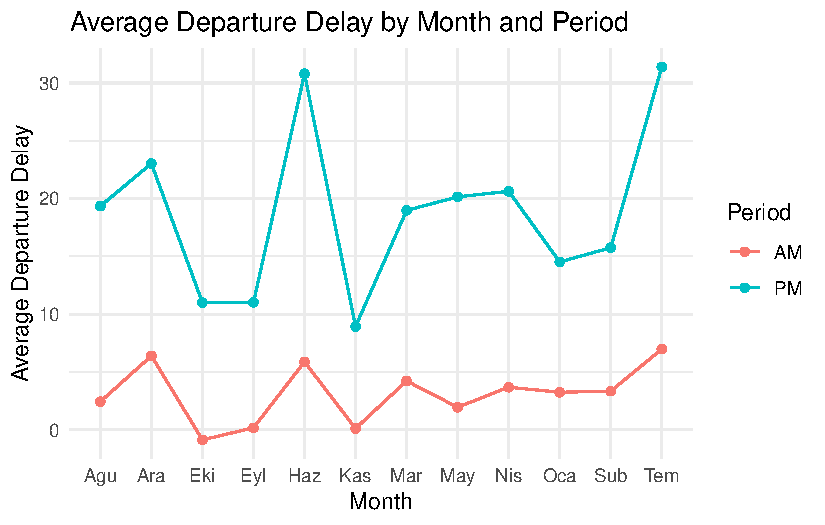
\includegraphics{STAT570_HW2_Date_Time_Components_files/figure-pdf/unnamed-chunk-11-1.pdf}

}

\end{figure}



\end{document}
